% docs/synthesis_report/synthesis_report.tex -- synthesis report for the LFU cache controller (rtl-v2-final).
% Supersedes the earlier Word report that quoted TSMC 28nm numbers without any source.
% Every number comes from results/P7/TABLES.md (committed files only): run
%   python3 -I docs/synthesis_report/gen_tables.py && python3 -I tools/paper_numbers_check.py docs/synthesis_report
% Plain numbers must appear in TABLES.md exactly; rounded numbers are written \rnd{shown}{source}.
\documentclass[11pt]{article}
\usepackage[T1]{fontenc}
\usepackage{mathptmx}
\usepackage{courier}
\usepackage[margin=1in,headheight=14pt]{geometry}
\usepackage{graphicx}
\usepackage{booktabs}
\usepackage{array}
\usepackage{url}
\usepackage{xcolor}
\usepackage{tikz}
\usetikzlibrary{positioning,arrows.meta,fit,calc}
\usepackage{fancyhdr}
\usepackage{enumitem}
\usepackage[skins]{tcolorbox}
\usepackage[font=small,labelfont=bf]{caption}
\usepackage[section]{placeins}
\usepackage[hidelinks]{hyperref}
\usepackage[final]{microtype}
\graphicspath{{figs/}}
\DeclareUrlCommand\src{\urlstyle{tt}}
\newcommand{\rnd}[2]{#1}
\setlist{itemsep=1pt,topsep=3pt}
\setlength{\emergencystretch}{1.5em}
\pagestyle{fancy}
\fancyhf{}
\fancyhead[L]{\small LFU cache controller: synthesis report}
\fancyhead[R]{\small NanGate45, not TSMC; pre-layout}
\fancyfoot[L]{\footnotesize area = sum of cell areas; no power analysis}
\fancyfoot[R]{\small\thepage}
\renewcommand{\headrulewidth}{0.4pt}
% generated by docs/synthesis_report/gen_tables.py from results/P7/TABLES.md; do not edit
\newcommand{\tabPFive}{%
\begin{tabular}{rrrrrrrrrr}
\toprule
Depth & Mode & Cells & FFs & Area & FF share & Fmax & WNS 1\,GHz & WNS 500\,MHz & Viol. \\
 & & & & ($\mu$m$^2$) & of area & (MHz) & (ns) & (ns) & 1G / 500M \\
\midrule
16 & 0 & 9,399 & 2,657 & \rnd{23,689}{23688.630} & \rnd{0.597}{0.5967} & \rnd{203}{203.1} & $-$\rnd{3.923}{3.9226} & $-$\rnd{2.923}{2.9226} & 0 / 0 \\
16 & 1 & 10,467 & 2,657 & \rnd{24,643}{24643.038} & \rnd{0.574}{0.5736} & \rnd{215}{215.1} & $-$\rnd{3.649}{3.6487} & $-$\rnd{2.649}{2.6487} & 2 / 2 \\
64 & 0 & 36,605 & 10,131 & \rnd{90,869}{90869.324} & \rnd{0.593}{0.5928} & \rnd{195}{194.7} & $-$\rnd{4.136}{4.1363} & $-$\rnd{3.136}{3.1363} & 0 / 0 \\
64 & 1 & 37,204 & 10,131 & \rnd{91,623}{91623.168} & \rnd{0.588}{0.5880} & \rnd{191}{190.5} & $-$\rnd{4.249}{4.2487} & $-$\rnd{3.249}{3.2487} & 2 / 2 \\
256 & 0 & 143,139 & 39,925 & \rnd{358,573}{358573.054} & \rnd{0.592}{0.5922} & \rnd{167}{167.4} & $-$\rnd{4.975}{4.9752} & $-$\rnd{3.975}{3.9752} & 18 / 18 \\
256 & 1 & 144,521 & 39,925 & \rnd{364,405}{364404.838} & \rnd{0.583}{0.5827} & \rnd{165}{165.3} & $-$\rnd{5.048}{5.0483} & $-$\rnd{4.048}{4.0483} & 130 / 130 \\
\bottomrule
\end{tabular}}
\newcommand{\sharePFive}{\rnd{0.574}{0.5736}--\rnd{0.597}{0.5967}}
\newcommand{\tabPFiveB}{%
\begin{tabular}{rrrrrrrrrr}
\toprule
Depth & Mode & Cells & FFs & Area & FF share & Fmax & WNS 1\,GHz & WNS 500\,MHz & Viol. \\
 & & & & ($\mu$m$^2$) & of area & (MHz) & (ns) & (ns) & 1G / 500M \\
\midrule
16 & 0 & 10,381 & 2,957 & \rnd{25,879}{25879.140} & \rnd{0.608}{0.6079} & \rnd{629}{629.2} & $-$\rnd{0.589}{0.5892} & met & 0 / 0 \\
16 & 1 & 10,690 & 2,957 & \rnd{26,137}{26137.160} & \rnd{0.602}{0.6019} & \rnd{624}{624.4} & $-$\rnd{0.602}{0.6015} & met & 1 / 1 \\
64 & 0 & 40,818 & 10,431 & \rnd{96,163}{96163.256} & \rnd{0.577}{0.5768} & \rnd{476}{476.1} & $-$\rnd{1.100}{1.1004} & $-$\rnd{0.272}{0.2720} & 17 / 19 \\
64 & 1 & 41,303 & 10,431 & \rnd{97,302}{97302.268} & \rnd{0.570}{0.5701} & \rnd{473}{472.6} & $-$\rnd{1.116}{1.1159} & $-$\rnd{0.295}{0.2950} & 2 / 2 \\
256 & 0 & 143,583 & 40,225 & \rnd{359,160}{359159.584} & \rnd{0.596}{0.5957} & \rnd{188}{188.4} & $-$\rnd{4.307}{4.3074} & $-$\rnd{3.307}{3.3074} & 64 / 64 \\
256 & 1 & 147,232 & 40,225 & \rnd{362,078}{362078.136} & \rnd{0.591}{0.5909} & \rnd{185}{185.2} & $-$\rnd{4.400}{4.3997} & $-$\rnd{3.400}{3.3997} & 83 / 83 \\
\bottomrule
\end{tabular}}
\newcommand{\sharePFiveB}{\rnd{0.570}{0.5701}--\rnd{0.609}{0.6094}}
\newcommand{\tabPFiveC}{%
\begin{tabular}{rrrrrrrrrr}
\toprule
Depth & Mode & Cells & FFs & Area & FF share & Fmax & WNS 1\,GHz & WNS 500\,MHz & Viol. \\
 & & & & ($\mu$m$^2$) & of area & (MHz) & (ns) & (ns) & 1G / 500M \\
\midrule
16 & 0 & 10,834 & 2,957 & \rnd{26,364}{26363.792} & \rnd{0.597}{0.5967} & \rnd{626}{626.1} & $-$\rnd{0.597}{0.5973} & met & 0 / 0 \\
16 & 1 & 11,242 & 2,957 & \rnd{26,634}{26634.048} & \rnd{0.591}{0.5906} & \rnd{612}{611.6} & $-$\rnd{0.635}{0.6351} & met & 0 / 0 \\
64 & 0 & 41,192 & 10,431 & \rnd{96,531}{96531.400} & \rnd{0.575}{0.5746} & \rnd{486}{486.4} & $-$\rnd{1.056}{1.0561} & $-$\rnd{0.308}{0.3076} & 8 / 7 \\
64 & 1 & 40,434 & 10,431 & \rnd{96,896}{96895.820} & \rnd{0.572}{0.5724} & \rnd{439}{439.3} & $-$\rnd{1.276}{1.2762} & $-$\rnd{0.349}{0.3492} & 9 / 5 \\
256 & 0 & 144,237 & 40,225 & \rnd{359,697}{359696.904} & \rnd{0.595}{0.5948} & \rnd{214}{213.9} & $-$\rnd{3.674}{3.6744} & $-$\rnd{2.674}{2.6744} & 118 / 118 \\
256 & 1 & 146,419 & 40,225 & \rnd{361,999}{361999.400} & \rnd{0.591}{0.5910} & \rnd{199}{199.4} & $-$\rnd{4.014}{4.0142} & $-$\rnd{3.014}{3.0142} & 48 / 48 \\
\bottomrule
\end{tabular}}
\newcommand{\sharePFiveC}{\rnd{0.572}{0.5724}--\rnd{0.598}{0.5982}}
\newcommand{\tabPFiveD}{%
\begin{tabular}{rrrrrrrrrr}
\toprule
Depth & Mode & Cells & FFs & Area & FF share & Fmax & WNS 1\,GHz & WNS 500\,MHz & Viol. \\
 & & & & ($\mu$m$^2$) & of area & (MHz) & (ns) & (ns) & 1G / 500M \\
\midrule
16 & 0 & 11,529 & 2,957 & \rnd{26,733}{26733.266} & \rnd{0.589}{0.5885} & \rnd{571}{571.3} & $-$\rnd{0.751}{0.7505} & met & 0 / 0 \\
16 & 1 & 11,661 & 2,957 & \rnd{26,875}{26875.310} & \rnd{0.585}{0.5853} & \rnd{587}{586.9} & $-$\rnd{0.704}{0.7040} & met & 1 / 1 \\
64 & 0 & 37,720 & 10,431 & \rnd{92,970}{92969.660} & \rnd{0.597}{0.5966} & \rnd{528}{528.4} & $-$\rnd{0.893}{0.8925} & $-$\rnd{0.179}{0.1794} & 2 / 3 \\
64 & 1 & 37,901 & 10,431 & \rnd{93,294}{93294.180} & \rnd{0.595}{0.5945} & \rnd{471}{470.9} & $-$\rnd{1.124}{1.1236} & $-$\rnd{0.340}{0.3400} & 3 / 3 \\
256 & 0 & 143,761 & 40,225 & \rnd{359,442}{359441.544} & \rnd{0.595}{0.5952} & \rnd{451}{451.2} & $-$\rnd{1.216}{1.2161} & $-$\rnd{0.343}{0.3432} & 120 / 120 \\
256 & 1 & 145,730 & 40,225 & \rnd{362,935}{362935.454} & \rnd{0.590}{0.5895} & \rnd{435}{435.3} & $-$\rnd{1.297}{1.2972} & $-$\rnd{0.337}{0.3366} & 108 / 131 \\
\bottomrule
\end{tabular}}
\newcommand{\sharePFiveD}{\rnd{0.585}{0.5853}--\rnd{0.597}{0.5971}}
\newcommand{\tabPFiveE}{%
\begin{tabular}{rrrrrrrrrr}
\toprule
Depth & Mode & Cells & FFs & Area & FF share & Fmax & WNS 1\,GHz & WNS 500\,MHz & Viol. \\
 & & & & ($\mu$m$^2$) & of area & (MHz) & (ns) & (ns) & 1G / 500M \\
\midrule
16 & 0 & 11,466 & 2,957 & \rnd{26,744}{26744.438} & \rnd{0.588}{0.5882} & \rnd{636}{636.1} & $-$\rnd{0.572}{0.5720} & met & 1 / 3 \\
16 & 1 & 11,057 & 2,957 & \rnd{26,627}{26626.866} & \rnd{0.591}{0.5908} & \rnd{660}{659.5} & $-$\rnd{0.516}{0.5162} & met & 1 / 1 \\
64 & 0 & 37,939 & 10,431 & \rnd{94,386}{94385.578} & \rnd{0.588}{0.5877} & \rnd{603}{603.0} & $-$\rnd{0.659}{0.6585} & met & 7 / 9 \\
64 & 1 & 38,692 & 10,431 & \rnd{95,101}{95100.852} & \rnd{0.583}{0.5832} & \rnd{611}{611.2} & $-$\rnd{0.636}{0.6360} & met & 6 / 8 \\
256 & 0 & 149,620 & 40,225 & \rnd{369,530}{369529.860} & \rnd{0.579}{0.5790} & \rnd{557}{556.6} & $-$\rnd{0.797}{0.7967} & $-$\rnd{0.036}{0.0357} & 61 / 100 \\
256 & 1 & 150,254 & 40,225 & \rnd{370,227}{370226.514} & \rnd{0.578}{0.5779} & \rnd{542}{542.3} & $-$\rnd{0.844}{0.8440} & $-$\rnd{0.002}{0.0015} & 19 / 23 \\
\bottomrule
\end{tabular}}
\newcommand{\sharePFiveE}{\rnd{0.578}{0.5779}--\rnd{0.593}{0.5929}}

% generated by docs/synthesis_report/gen_tables.py from results/P7/TABLES.md; do not edit
\newcommand{\cpStartBaseSixteen}{\texttt{freq\_cnt[1][0]}}\newcommand{\cpEndBaseSixteen}{\texttt{valid\_bits[9]}}
\newcommand{\cpSumBaseSixteen}{114 & \rnd{4.879}{4.8791} & $-$\rnd{3.923}{3.9226} & 10 / \rnd{0.486}{0.4855} & 1 / \rnd{0.036}{0.0355} & \rnd{4.393}{4.3934}}
\newcommand{\cpTypesBaseSixteen}{AOI22\_X1 32$\times$, \rnd{1.407}{1.4065}; OAI22\_X1 26$\times$, \rnd{0.725}{0.7251}; MUX2\_X1 10$\times$, \rnd{0.644}{0.6435}; OAI21\_X1 8$\times$, \rnd{0.351}{0.3507}; AOI21\_X1 4$\times$, \rnd{0.247}{0.2468}; BUF\_X2 5$\times$, \rnd{0.219}{0.2193}}
\newcommand{\cpStartBaseTwoFiveSix}{\texttt{req\_addr\_reg[4]}}\newcommand{\cpEndBaseTwoFiveSix}{\texttt{freq\_cnt[1][0]}}
\newcommand{\cpSumBaseTwoFiveSix}{87 & \rnd{5.934}{5.9343} & $-$\rnd{4.975}{4.9752} & 58 / \rnd{4.358}{4.3580} & 52 / \rnd{3.933}{3.9331} & \rnd{1.576}{1.5760}}
\newcommand{\cpTypesBaseTwoFiveSix}{BUF\_X1 57$\times$, \rnd{4.268}{4.2683}; NOR4\_X1 4$\times$, \rnd{0.472}{0.4722}; OAI21\_X1 6$\times$, \rnd{0.189}{0.1885}; OR4\_X1 1$\times$, \rnd{0.135}{0.1347}; AOI21\_X1 6$\times$, \rnd{0.123}{0.1226}; NOR3\_X1 1$\times$, \rnd{0.121}{0.1213}}
\newcommand{\cpStartFinalSixteen}{\texttt{freq\_cnt[9][1]}}\newcommand{\cpEndFinalSixteen}{\texttt{victim\_reg[0]}}
\newcommand{\cpSumFinalSixteen}{26 & \rnd{1.537}{1.5368} & $-$\rnd{0.572}{0.572} & 4 / \rnd{0.145}{0.1451} & 1 / \rnd{0.046}{0.0464} & \rnd{1.392}{1.3920}}
\newcommand{\cpTypesFinalSixteen}{AOI221\_X1 2$\times$, \rnd{0.229}{0.2293}; OAI221\_X1 3$\times$, \rnd{0.176}{0.1756}; MUX2\_X1 2$\times$, \rnd{0.137}{0.1371}; OAI33\_X1 1$\times$, \rnd{0.128}{0.1276}; DFFR\_X1 1$\times$, \rnd{0.098}{0.0983}; OAI221\_X4 1$\times$, \rnd{0.093}{0.0926}}
\newcommand{\cpStartFinalTwoFiveSix}{\texttt{freq\_cnt[207][1]}}\newcommand{\cpEndFinalTwoFiveSix}{\texttt{stageA\_min[12][1]}}
\newcommand{\cpSumFinalTwoFiveSix}{29 & \rnd{1.760}{1.7598} & $-$\rnd{0.797}{0.7967} & 3 / \rnd{0.207}{0.2072} & 1 / \rnd{0.067}{0.0672} & \rnd{1.553}{1.5526}}
\newcommand{\cpTypesFinalTwoFiveSix}{AOI221\_X1 4$\times$, \rnd{0.282}{0.2824}; MUX2\_X1 3$\times$, \rnd{0.222}{0.2217}; BUF\_X1 3$\times$, \rnd{0.207}{0.2072}; AND2\_X1 3$\times$, \rnd{0.154}{0.1542}; OR4\_X1 1$\times$, \rnd{0.118}{0.1180}; NAND4\_X1 2$\times$, \rnd{0.112}{0.1120}}

% generated by docs/synthesis_report/gen_tables.py from results/P7/TABLES.md; do not edit
\newcommand{\mcpTable}{%
\begin{tabular}{rrrrrrr}
\toprule
 & & & \multicolumn{2}{c}{Old flow WNS (ns)} & \multicolumn{2}{c}{Timing-driven WNS (ns)} \\
\cmidrule(lr){4-5}\cmidrule(lr){6-7}
Depth & Mode & MHz & without & with & without & with \\
\midrule
16 & 0 & 1000 & $-$\rnd{0.751}{0.7505} & $-$\rnd{0.719}{0.7187} & $-$\rnd{0.572}{0.5720} & $-$\rnd{0.554}{0.5540} \\
16 & 0 & 500 & 0 & 0 & 0 & 0 \\
16 & 1 & 1000 & $-$\rnd{0.704}{0.7040} & $-$\rnd{0.694}{0.6936} & $-$\rnd{0.516}{0.5162} & $-$\rnd{0.490}{0.4903} \\
16 & 1 & 500 & 0 & 0 & 0 & 0 \\
64 & 0 & 1000 & $-$\rnd{0.893}{0.8925} & $-$\rnd{0.893}{0.8925} & $-$\rnd{0.659}{0.6585} & $-$\rnd{0.652}{0.6524} \\
64 & 0 & 500 & $-$\rnd{0.179}{0.1794} & $-$\rnd{0.179}{0.1794} & 0 & 0 \\
64 & 1 & 1000 & $-$\rnd{1.124}{1.1236} & $-$\rnd{1.096}{1.0964} & $-$\rnd{0.636}{0.6360} & $-$\rnd{0.635}{0.6345} \\
64 & 1 & 500 & $-$\rnd{0.340}{0.3400} & $-$\rnd{0.277}{0.2772} & 0 & 0 \\
256 & 0 & 1000 & $-$\rnd{1.216}{1.2161} & $-$\rnd{1.216}{1.2161} & $-$\rnd{0.797}{0.7967} & $-$\rnd{0.792}{0.7918} \\
256 & 0 & 500 & $-$\rnd{0.343}{0.3432} & $-$\rnd{0.343}{0.3432} & $-$\rnd{0.036}{0.0357} & $-$\rnd{0.036}{0.0357} \\
256 & 1 & 1000 & $-$\rnd{1.297}{1.2972} & $-$\rnd{1.291}{1.2911} & $-$\rnd{0.844}{0.8440} & $-$\rnd{0.844}{0.8440} \\
256 & 1 & 500 & $-$\rnd{0.337}{0.3366} & $-$\rnd{0.326}{0.3262} & $-$\rnd{0.002}{0.0015} & $-$0.0001 \\
\bottomrule
\end{tabular}}
\newcommand{\mcpMaxOld}{\rnd{0.063}{0.0628}}\newcommand{\mcpMaxNew}{\rnd{0.026}{0.0259}}

% generated by docs/synthesis_report/gen_tables.py from results/P7/TABLES.md; do not edit
\newcommand{\cidFinal}{\texttt{7705a7b}}
\newcommand{\cidBase}{\texttt{0d66a3a}}
\newcommand{\cidPfiveB}{\texttt{4debe84}}
\newcommand{\cidPfiveC}{\texttt{73016e0}}
\newcommand{\cidFlow}{\texttt{b69a931}}
\newcommand{\cidGls}{\texttt{02518be}}
\newcommand{\cidTables}{\texttt{f0f82ce}}
\newcommand{\fileIndex}{%
\begin{tabular}{>{\raggedright\arraybackslash}p{0.44\textwidth}>{\raggedright\arraybackslash}p{0.245\textwidth}ll}
\toprule
File & Content & Added in & Last changed \\
\midrule
\src{results/P5/RESULTS.md} & P5 baseline, all runs & \texttt{b5d85b7} & \texttt{b5d85b7} \\
\src{results/P5/SOURCES.md} & toolchain and liberty record & \texttt{b5d85b7} & \texttt{b5d85b7} \\
\src{results/P5/CRITICAL_PATH.md} & baseline critical paths & \texttt{99cdde6} & \texttt{0d66a3a} \\
\src{results/P5b/RESULTS.md} & P5b runs & \texttt{4debe84} & \texttt{73016e0} \\
\src{results/P5c/tree_copies/RESULTS.md} & P5c runs (kept variant) & \texttt{73016e0} & \texttt{73016e0} \\
\src{results/P5c/tree_only/RESULTS.md} & P5c tree only & \texttt{73016e0} & \texttt{73016e0} \\
\src{results/P5d/RESULTS.md} & P5d runs (rtl-v2-final, old flow) & \texttt{7705a7b} & \texttt{7705a7b} \\
\src{results/P5d/NOISE.md} & old-flow noise floor & \texttt{7705a7b} & \texttt{7705a7b} \\
\src{results/P5d/mutation.txt} & mutation test of the final RTL & \texttt{7705a7b} & \texttt{7705a7b} \\
\src{results/P5e/new/RESULTS.md} & P5e runs (final) & \texttt{b69a931} & \texttt{b69a931} \\
\src{results/P5e/COMPARE.md} & flow comparison, noise, multicycle & \texttt{b69a931} & \texttt{b69a931} \\
\src{results/P5e/CRITICAL_PATH.md} & final critical paths & \texttt{b69a931} & \texttt{b69a931} \\
\src{results/P5f_gls/CELLCHECK.md} & cell-model check & \texttt{4188580} & \texttt{4188580} \\
\src{results/P5f_gls/COVERAGE.md} & cell-type coverage & \texttt{4188580} & \texttt{4188580} \\
\src{results/P5f_gls/equiv/} & depth-16 equivalence & \texttt{42a8201} & \texttt{42a8201} \\
\src{results/P5f_gls/cluster/} & cluster gate-level runs & \texttt{02518be} & \texttt{02518be} \\
\src{results/P5f_gls/sim/} & local gate-level unit tests & \texttt{4188580} & \texttt{4188580} \\
\src{results/P5f_gls/SUMMARY.md} & gate-level summary & \texttt{02518be} & \texttt{061f0cf} \\
\src{results/P7/TABLES.md} & all tables, generated & \texttt{1575c09} & \texttt{f0f82ce} \\
\src{results/COMMIT_MAP.md} & old-to-new commit IDs & \texttt{061f0cf} & \texttt{061f0cf} \\
\bottomrule
\end{tabular}}


\title{Synthesis Report: LFU Cache Controller \texttt{rtl-v2-final} on NanGate45\\[4pt]
\large NanGate45, not TSMC; pre-layout; area = sum of cell areas; no power analysis}
\author{Adarsh\\ \small Department of Electrical and Electronics Engineering\\ \small BITS Pilani, K K Birla Goa Campus,
Goa, India \and Pravin Mane\\ \small Department of Electrical and Electronics Engineering\\ \small BITS Pilani, K K
Birla Goa Campus, Goa, India}
\date{}

\begin{document}
\maketitle
\thispagestyle{fancy}

\begin{tcolorbox}[colback=black!4,colframe=black!60,boxrule=0.6pt,arc=1pt,left=6pt,right=6pt,top=4pt,bottom=4pt,
  title={\textbf{1. Scope and limits: read this first}},coltitle=black,colbacktitle=black!12]
\textbf{What this report is.} Logic synthesis (Yosys and ABC) and static timing analysis (OpenSTA) of the LFU cache
controller of tag \texttt{rtl-v2-final}, mapped to the NanGate45 open cell library, with functional verification of
the resulting netlists. Every number is taken from committed result files through \src{results/P7/TABLES.md}
(commit \cidTables) and checked by \src{tools/paper_numbers_check.py}.

\textbf{What it is not.}
\begin{itemize}[leftmargin=12pt]
\item \textbf{Not TSMC.} NanGate45 is an open library for a generic predictive process. This report supersedes an
earlier Word report whose TSMC 28nm area, power and timing figures have no source file; none of them is used here.
\item \textbf{Pre-layout.} Interconnect is estimated by the liberty wire-load model; the clock is ideal (no clock tree);
there is no placement, routing or parasitic extraction.
\item \textbf{Area} is the sum of the liberty cell areas, not a placed area. Storage is built from flip-flops; there is
no SRAM macro.
\item \textbf{No power analysis} was run, so this report contains no power numbers.
\item \textbf{Gate-level simulation is zero-delay} (no SDF), with cell models generated by Yosys from the liberty file;
formal equivalence is proven at depth 16 only.
\item \textbf{Flow noise.} Synthesizing identical logic in different textual forms moves Fmax by 1.96--16.62\% (earlier
flow) and 4.92--16.23\% (current flow); differences smaller than that are not evidence of a design effect.
\end{itemize}
\end{tcolorbox}

\addcontentsline{toc}{section}{\protect\numberline{1}Scope and limits}
{\small\setcounter{tocdepth}{1}\tableofcontents}

\setcounter{section}{1}
\section{Design}
\textbf{RTL.} \src{rtl/v2/lfu_cache_controller.v} at tag \texttt{rtl-v2-final} (commit \cidFinal). The file in the
repository is identical to the tag (checked by \src{tools/make_tables.py}).

\textbf{Parameters.} Address width 20 bits, vector width 128 bits, counter width 6 bits (saturating at 63), 16 groups
for victim selection. Synthesized at depths (\texttt{CACHE\_DEPTH}) 16, 64 and 256 lines.

\textbf{Counter modes} (parameter \texttt{COUNTER\_MODE}). Mode~0, the default, sets the count of a newly
installed tag to one; mode~1 lets the new tag continue from the count left in the slot. Mode~2 (per-address history) is not
implemented: elaboration stops with an error. Both implemented modes are synthesized.

\begin{figure}[h]
\centering
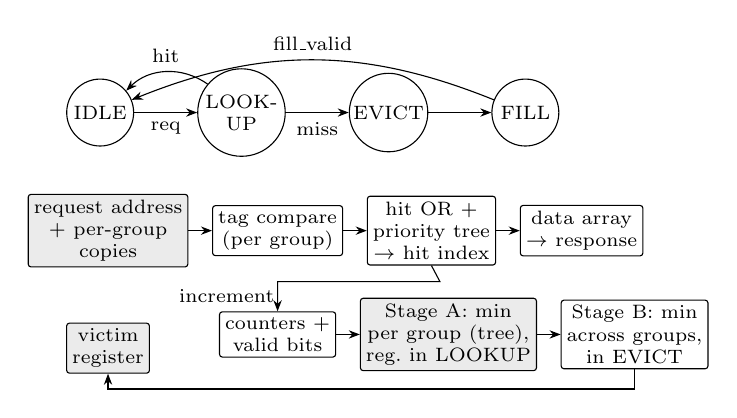
\begin{tikzpicture}[
  font=\scriptsize, >={Stealth[length=4pt]},
  blk/.style={draw, rounded corners=1pt, align=center, minimum height=5.5mm, inner sep=2pt, fill=white},
  st/.style={draw, circle, inner sep=1pt, minimum size=8.5mm, align=center},
  reg/.style={blk, fill=black!8}]
  % FSM
  \node[st] (idle) {IDLE};
  \node[st, right=8mm of idle] (look) {LOOK-\\UP};
  \node[st, right=8mm of look] (evict) {EVICT};
  \node[st, right=8mm of evict] (fill) {FILL};
  \draw[->] (idle) -- node[below]{req} (look);
  \draw[->] (look) -- node[below]{miss} (evict);
  \draw[->] (evict) -- (fill);
  \draw[->] (look) to[bend right=40] node[above]{hit} (idle);
  \draw[->] (fill) to[bend right=22] node[above]{fill\_valid} (idle);
  % datapath
  \node[reg, below=6mm of idle, xshift=1mm] (addr) {request address\\+ per-group\\copies};
  \node[blk, right=3mm of addr] (cmp) {tag compare\\(per group)};
  \node[blk, right=3mm of cmp] (hit) {hit OR +\\priority tree\\$\rightarrow$ hit index};
  \node[blk, right=3mm of hit] (data) {data array\\$\rightarrow$ response};
  \node[blk, below=7mm of cmp] (cnt) {counters +\\valid bits};
  \node[reg, right=3mm of cnt] (sa) {Stage A: min\\per group (tree),\\reg.\ in LOOKUP};
  \node[blk, right=3mm of sa] (sb) {Stage B: min\\across groups,\\in EVICT};
  \node[reg, below=7mm of addr] (vic) {victim\\register};
  \draw[->] (addr) -- (cmp);
  \draw[->] (cmp) -- (hit);
  \draw[->] (hit) -- (data);
  \draw[->] (cnt) -- (sa);
  \draw[->] (sa) -- (sb);
  \draw[->] (sb.south) -- ++(0,-2.5mm) -| (vic.south);
  \coordinate (mid) at ($(hit.south)!0.5!(sa.north)$);
  \draw[->] (hit.south) -- (mid) -| node[pos=0.75, left, inner sep=1pt]{increment} (cnt.north);
\end{tikzpicture}
\caption[]{The LFU controller: FSM (top) and datapath (bottom; shaded blocks are registers). A hit returns to
IDLE; a miss selects the victim (Stage A registered in LOOKUP, Stage B in EVICT) and installs the fill in FILL.}
\label{fig:rtl}
\end{figure}

\textbf{Operation} (Fig.~\ref{fig:rtl}). A request moves the FSM from IDLE to LOOKUP. The tag compare runs per group on
registered copies of the request address; a per-group OR and a balanced priority tree give the lowest matching line
(the \emph{hit path}). On a hit the line's counter is incremented and the vector is returned. On a miss the victim is
the line with the smallest count: \textbf{Stage~A} is a reduction tree inside each group, registered at the end of
LOOKUP; \textbf{Stage~B} is a reduction tree across the 16 group minima, evaluated in EVICT, whose result is written to
the victim register; an invalid line counts as smaller than any valid one, and ties go to the lower slot index. FILL
writes the returned vector, the tag and the new count into the victim slot.

\section{Toolchain and reproducibility}
\begin{center}\small
\begin{tabular}{>{\raggedright\arraybackslash}p{0.25\textwidth}>{\raggedright\arraybackslash}p{0.69\textwidth}}
\toprule
Item & Version / identifier \\
\midrule
Yosys & 0.33, git \texttt{2584903a060} \\
ABC & the copy built into Yosys 0.33 (no separate version recorded) \\
OpenSTA & 3.1.0, commit\newline \texttt{7b261909c1730d963252142e136daaa0199e333c} \\
CUDD (OpenSTA dependency) & tag \texttt{3.0.0}, commit\newline \texttt{f54f533303640afd5dbe47a05ebeabb3066f2a25} \\
Liberty & \texttt{NangateOpenCellLibrary\_typical.lib}, corner typical, 25C, 1.1V \\
\quad source & OpenROAD-flow-scripts, commit\newline \texttt{6c6fc7e21b2d0b5b88b1a52d0a5860ea4d88e9e5} \\
\quad sha256 & {\scriptsize\texttt{8d540a4d4cf6d09d27c87ad067857a9c0c2eeb023ab7a56e058cd3113db4e9b1}} \\
\quad size & 6,692,032 bytes (not redistributed; see \src{results/P5/SOURCES.md} for its licence header) \\
Icarus Verilog & 12.0 (local), 11.0 (cluster) \\
\bottomrule
\end{tabular}
\end{center}
Sources: \src{results/P5/SOURCES.md} (build record of the local tools), the cluster gate-level logs and
\src{results/P5f_gls/jobs.txt}; all collected in \src{results/P7/TABLES.md}, section ``Flow settings and toolchain''.
Flow scripts: \src{synthesis/p5/} (synthesis template, ABC constraints, STA script, driver), \src{synthesis/p5e/}
(timing-driven ABC script and template, multicycle STA), \src{synthesis/p5c/}, \src{synthesis/p5d/} (design-iteration
drivers), \src{synthesis/p5f/} (gate-level simulation). The commands that regenerate every table are listed in the
appendix.

\section{Flow}
\textbf{Synthesis} (\src{synthesis/p5/synth.ys.in}): read the liberty as a cell library, read the RTL, set depth and
counter mode, \texttt{proc}, copy the \texttt{keep} attribute onto the flip-flops that drive the per-group address
copies (otherwise Yosys merges the identical registers), \texttt{synth -flatten}, \texttt{dfflibmap} to the liberty
flip-flops, \texttt{abc} technology mapping, tie cells, \texttt{stat -liberty} (cell counts and area) and
\texttt{check -assert}.

\textbf{ABC.} The earlier flow (P5--P5d) calls \texttt{abc -liberty -D <period> -constr}, i.e.\ Yosys's built-in
script. The current flow (P5e, \src{synthesis/p5e/abc_td.script.in}) runs three delay-oriented restructuring passes
(\texttt{\&st; \&syn2; \&if -g -K 6; \&synch2; \&nf -D}), then buffering including flip-flop outputs
(\texttt{buffer -c -p}) and gate sizing (\texttt{upsize -c}, \texttt{dnsize -c}), all with the liberty's wire-load
model. Its delay target is the clock period minus 141.5\,ps: ABC sees flip-flop outputs as inputs and flip-flop inputs
as outputs, so clock-to-Q and setup are subtracted beforehand; 141.5\,ps is clk$\rightarrow$Q 0.0983\,ns plus setup
0.0432\,ns on the worst path of the earlier flow's depth-16, mode-0, 1\,GHz run.

\textbf{Constraints.} Inputs driven by a BUF\_X1 cell and outputs loaded with 3.795620\,fF, the same in ABC and in STA.

\textbf{STA} (\src{synthesis/p5/sta.tcl}). Wire-load model 5K\_hvratio\_1\_1; ideal clock; input and output delay 0
relative to the clock; the asynchronous reset's recovery and removal paths are excluded
(\texttt{set\_false\_path -from rst\_n}), because the reset net has no buffer tree before layout; its slew and
capacitance violation is still reported but not counted below. Multicycle exceptions are used only in the cross-check
of Section~\ref{sec:issues}; all headline numbers use none.

\textbf{Fmax} $=1/(T-\mathrm{WNS})$ from the worst setup path of the netlist synthesized for a period $T$; ``met'' means
WNS $\ge 0$. Each configuration is synthesized twice, for 1\,GHz and for 500\,MHz.

\section{Results}\label{sec:results}
One table per design iteration. Cells, flip-flops (FFs), area, flip-flop share of area and Fmax are from the 1\,GHz
netlist; ``WNS 500\,MHz'' is from the netlist synthesized for 500\,MHz; ``Viol.'' counts nets or pins that violate a
max-slew or max-capacitance limit in the 1\,GHz / 500\,MHz netlists (reset net excluded). Values are rounded for display
(area and Fmax to integers, slack to 3 decimals); the unrounded values are in \src{results/P7/TABLES.md}.

\begin{table}[h]\centering\small
\caption[]{P5 baseline (tag \texttt{rtl-v2-baseline}, commit \cidBase): serial minimum and priority loops; earlier flow.
The 1\,GHz and 500\,MHz netlists are identical at every depth (the ABC target did not bind).}
\setlength{\tabcolsep}{4pt}\tabPFive
\end{table}
\begin{table}[h]\centering\small
\caption[]{P5b (commit \cidPfiveB): Stage-B reduction tree and per-group address copies; earlier flow.}
\setlength{\tabcolsep}{4pt}\tabPFiveB
\end{table}
\begin{table}[h]\centering\small
\caption[]{P5c (commit \cidPfiveC): Stage-A reduction tree, with the address copies kept; earlier flow.}
\setlength{\tabcolsep}{4pt}\tabPFiveC
\end{table}
\begin{table}[h]\centering\small
\caption[]{P5d (tag \texttt{rtl-v2-final}, commit \cidFinal): hit-index priority tree; earlier flow.}
\setlength{\tabcolsep}{4pt}\tabPFiveD
\end{table}
\begin{table}[h]\centering\small
\caption[]{P5e (same RTL, \texttt{rtl-v2-final}; flow commit \cidFlow): timing-driven ABC flow. These are the current
numbers of the controller.}
\setlength{\tabcolsep}{4pt}\tabPFiveE
\end{table}

\begin{figure}[h]\centering
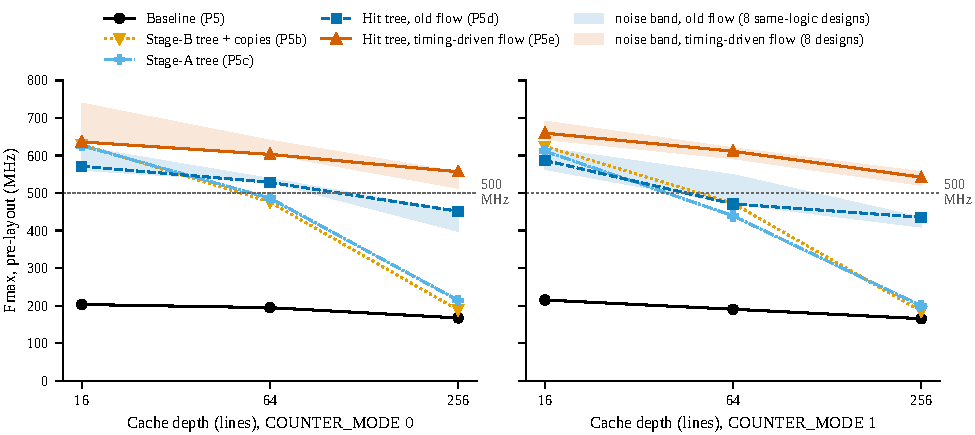
\includegraphics{fig_fmax}
\caption[]{Pre-layout Fmax of the 1\,GHz netlists vs.\ depth for each design iteration, with the flow noise bands
(min--max Fmax of 8 designs with identical logic) for the earlier and the timing-driven flow. Script
\src{paper/v2/figs/fig_fmax.py} (the paper's figure at report width).}
\label{fig:fmax}
\end{figure}

\textbf{Summary.} The final design reaches \rnd{636}{636.1}, \rnd{603}{603.0} and \rnd{557}{556.6}\,MHz at depths 16,
64 and 256 in mode~0, and \rnd{660}{659.5}, \rnd{611}{611.2} and \rnd{542}{542.3}\,MHz in mode~1. The 500\,MHz netlists
meet 500\,MHz at depths 16 and 64; at depth 256 they miss by \rnd{0.036}{0.0357}\,ns (mode 0) and \rnd{0.002}{0.0015}\,ns
(mode 1), far inside the 8.53\% and 7.02\% noise spread at that depth, so meeting 500\,MHz at depth 256 is not
demonstrated either way. Flip-flops take \sharePFiveE{} of the cell area in the final design (\sharePFive{} in the
baseline).

\section{Critical paths}\label{sec:paths}
Worst setup path of the 1\,GHz netlists, mode~0, for the baseline and the final design at depths 16 and 256.
\textbf{Tool output} (OpenSTA \texttt{report\_checks}, per-cell rows): start and end registers, number of cells, arrival,
slack, buffers, per-cell-type delays. The register names were mapped from flip-flop instances to RTL registers by
\src{tools/p5_critical_path.py} using the netlists. \textbf{My reading} (not tool output): which RTL structure the
path belongs to, and whether it can occur in one clock cycle.

\noindent\textbf{Start $\rightarrow$ end registers} (tool output):
\begin{itemize}[leftmargin=14pt]
\item Baseline, depth 16: \cpStartBaseSixteen{} $\rightarrow$ \cpEndBaseSixteen.
\item Baseline, depth 256: \cpStartBaseTwoFiveSix{} $\rightarrow$ \cpEndBaseTwoFiveSix.
\item Final, depth 16: \cpStartFinalSixteen{} $\rightarrow$ \cpEndFinalSixteen.
\item Final, depth 256: \cpStartFinalTwoFiveSix{} $\rightarrow$ \cpEndFinalTwoFiveSix.
\end{itemize}

\begin{table}[h]\centering\small
\caption[]{Critical-path summary (tool output). Cells include the launching flip-flop. Delays in ns; slack at 1\,GHz.}
\begin{tabular}{lrrrrrr}
\toprule
Path & Cells & Arrival & Slack & Buffers & Longest buffer run & Non-buffer \\
 & & & & count / delay & cells / delay & delay \\
\midrule
Baseline, depth 16 & \cpSumBaseSixteen \\
Baseline, depth 256 & \cpSumBaseTwoFiveSix \\
Final, depth 16 & \cpSumFinalSixteen \\
Final, depth 256 & \cpSumFinalTwoFiveSix \\
\bottomrule
\end{tabular}
\end{table}

\noindent\textbf{Largest delay contributions by cell type} (tool output; count and summed delay in ns, six largest):
\begin{itemize}[leftmargin=14pt]
\item Baseline, depth 16: \cpTypesBaseSixteen.
\item Baseline, depth 256: \cpTypesBaseTwoFiveSix.
\item Final, depth 16: \cpTypesFinalSixteen.
\item Final, depth 256: \cpTypesFinalTwoFiveSix.
\end{itemize}

\noindent\textbf{What the paths are} (my reading of the netlist against the RTL, not tool output):
\begin{itemize}[leftmargin=14pt]
\item \emph{Baseline, depth 16}: Stage-B victim selection in EVICT, then the write that clears the victim's valid bit.
In the baseline, Stage B was a serial loop over the 16 group minima; with 16 groups at depth 16 each group has one
line, so the whole minimum search is this serial compare-and-select chain (the repeated AOI22/OAI22 pairs and MUX2
cells).
\item \emph{Baseline, depth 256}: the hit path in LOOKUP: registered request address $\rightarrow$ tag compare $\rightarrow$
priority loop for the hit index $\rightarrow$ counter increment. Most of its delay is a serial run of 52 buffers that
ABC's buffering built on the high-fanout address net; the logic itself is short.
\item \emph{Final, depth 16}: victim selection into the victim register (Stage-B tree; at depth 16 Stage A has one line
per group). The counters change only on edges into IDLE, and the victim register loads only in EVICT, at least three
cycles later, so this path cannot be exercised in one cycle (Section~\ref{sec:issues}).
\item \emph{Final, depth 256}: counter $\rightarrow$ Stage-A minimum register (the Stage-A tree, registered at the end
of LOOKUP). The counters change only on edges into IDLE, and the Stage-A register loads at the end of LOOKUP, at
least two cycles later, so this is also not a one-cycle path. With the multicycle
exceptions the worst path becomes a Stage-A register $\rightarrow$ valid bit through Stage B (tool output of the
cross-check run).
\end{itemize}

\section{Flow noise floor}\label{sec:noise}
Eight designs with identical logic were synthesized with each flow at 1\,GHz: the final RTL, a flat-vector (``packed'')
form of the same hit tree, and three one-line rewrites of each (swapped operands of the tag compare and of the hit-tree
OR, and a comparison written the other way round; \src{tools/p5d_null_variants.py}). Any spread in their Fmax is
variation of the flow, not of the design. Spread = max/min $-$ 1.
\begin{center}\small% generated by docs/synthesis_report/gen_tables.py from results/P7/TABLES.md; do not edit
\begin{tabular}{rrrrrr}
\toprule
 & & \multicolumn{2}{c}{Old flow (P5d)} & \multicolumn{2}{c}{Timing-driven flow (P5e)} \\
\cmidrule(lr){3-4}\cmidrule(lr){5-6}
Depth & Mode & Fmax min--max (MHz) & Spread & Fmax min--max (MHz) & Spread \\
\midrule
16 & 0 & \rnd{561}{560.7}--\rnd{623}{623.0} & 11.12\% & \rnd{636}{636.1}--\rnd{739}{739.4} & 16.23\% \\
16 & 1 & \rnd{563}{563.1}--\rnd{621}{620.5} & 10.20\% & \rnd{642}{642.2}--\rnd{692}{691.8} & 7.71\% \\
64 & 0 & \rnd{528}{528.4}--\rnd{539}{538.8} & 1.96\% & \rnd{603}{603.0}--\rnd{641}{640.6} & 6.24\% \\
64 & 1 & \rnd{471}{470.9}--\rnd{549}{549.1} & 16.62\% & \rnd{591}{591.4}--\rnd{621}{620.5} & 4.92\% \\
256 & 0 & \rnd{398}{397.9}--\rnd{452}{451.8} & 13.54\% & \rnd{513}{512.8}--\rnd{557}{556.6} & 8.53\% \\
256 & 1 & \rnd{409}{409.0}--\rnd{435}{435.3} & 6.42\% & \rnd{520}{520.4}--\rnd{557}{556.9} & 7.02\% \\
\bottomrule
\end{tabular}
\end{center}

\section{Verification}\label{sec:verif}
\textbf{RTL.} A self-checking testbench with 7 tests passes at every depth and mode. Each RTL version was compared in
lockstep with the earlier versions on random traffic: every run in the eight lockstep result files of P5b--P5d (six
runs each, 200,000 cycles) passed with 0 port and 0 victim-slot mismatches, and 0 hit-index mismatches in the P5d files,
the only ones that record them. Mutation testing of the final RTL:
113 mutant runs killed by the unit tests, 10 more by the lockstep check, 33 runs of equivalent mutants; result ``OK
(all non-equivalent mutants killed)''.

\textbf{Cell models.} The gate-level simulation uses cell models generated by Yosys from the liberty file. They were
checked against the liberty functions by exhaustive truth tables (combinational cells) and random stimulus
(flip-flops): 84 cells pass, 1 fails. The failing cell is DFFRS\_X1 (flip-flop with asynchronous clear and preset),
whose generated model differs from the liberty function when clear and preset are both active and when one of them is
released while the other is still active; no netlist uses DFFRS\_X1. The netlists use 84
distinct cell types, all with a model that passed; there are no scan flip-flops.

\textbf{Gate-level lockstep} (functional, zero delay; Icarus 11.0 on the cluster). Each of the 12 netlists runs the
same 200,000 random cycles as the RTL; hit flag, response valid, response data, fill request and fill address are
compared every cycle. Result: 0 mismatching cycles and no X on any output in all 12. An RTL rerun of the same stimulus
shows that it drives counters to their maximum of 63 in every depth and mode (\src{results/P7/counter_sat/}).
\begin{center}\small% generated by docs/synthesis_report/gen_tables.py from results/P7/TABLES.md; do not edit
\begin{tabular}{rrrrrrrrrr}
\toprule
Depth & Mode & MHz & Cycles & Hits & Misses & Mismatch & X (gl/rtl) & vvp wall & Peak RSS (kB) \\
\midrule
16 & 0 & 1000 & 200000 & 57297 & 8139 & 0 & 0/0 & 7:53.04 & 65392 \\
16 & 0 & 500 & 200000 & 57297 & 8139 & 0 & 0/0 & 8:16.61 & 65472 \\
16 & 1 & 1000 & 200002 & 57090 & 8166 & 0 & 0/0 & 8:11.14 & 64680 \\
16 & 1 & 500 & 200002 & 57090 & 8166 & 0 & 0/0 & 7:43.67 & 64860 \\
64 & 0 & 1000 & 200000 & 57092 & 8199 & 0 & 0/0 & 25:07.54 & 212308 \\
64 & 0 & 500 & 200000 & 57092 & 8199 & 0 & 0/0 & 25:11.24 & 212688 \\
64 & 1 & 1000 & 200000 & 53588 & 9369 & 0 & 0/0 & 25:21.85 & 215572 \\
64 & 1 & 500 & 200000 & 53588 & 9369 & 0 & 0/0 & 24:32.00 & 215580 \\
256 & 0 & 1000 & 200000 & 57209 & 8109 & 0 & 0/0 & 1:37:59.46 & 819684 \\
256 & 0 & 500 & 200000 & 57209 & 8109 & 0 & 0/0 & 1:39:11.79 & 819572 \\
256 & 1 & 1000 & 200000 & 56927 & 8216 & 0 & 0/0 & 1:40:56.35 & 825804 \\
256 & 1 & 500 & 200000 & 56927 & 8216 & 0 & 0/0 & 1:40:07.57 & 825892 \\
\bottomrule
\end{tabular}
\end{center}

\textbf{Unit tests on the netlists.} The 7-test testbench, unmodified, on the depth-16 and depth-64 netlists with
Icarus 12.0 (local) and on the depth-16 and depth-256 netlists with Icarus 11.0 (cluster): 16 runs, all pass.
\begin{center}\small% generated by docs/synthesis_report/gen_tables.py from results/P7/TABLES.md; do not edit
\begin{tabular}{rrrlrll}
\toprule
Depth & Mode & MHz & Where & Result & Compile & Run \\
\midrule
16 & 0 & 1000 & local & pass & 5.14 s & 32.94 s \\
16 & 0 & 500 & local & pass & 3.32 s & 30.20 s \\
16 & 1 & 1000 & local & pass & 3.58 s & 28.74 s \\
16 & 1 & 500 & local & pass & 3.63 s & 29.21 s \\
64 & 0 & 1000 & local & pass & 73.16 s & 96.20 s \\
64 & 0 & 500 & local & pass & 57.07 s & 98.71 s \\
64 & 1 & 1000 & local & pass & 54.71 s & 112.18 s \\
64 & 1 & 500 & local & pass & 56.23 s & 113.59 s \\
16 & 0 & 1000 & cluster & pass & 0:01.92 & 0:11.67 \\
16 & 0 & 500 & cluster & pass & 0:02.03 & 0:11.81 \\
16 & 1 & 1000 & cluster & pass & 0:01.93 & 0:11.98 \\
16 & 1 & 500 & cluster & pass & 0:02.01 & 0:11.93 \\
256 & 0 & 1000 & cluster & pass & 13:03.75 & 7:02.92 \\
256 & 0 & 500 & cluster & pass & 13:09.11 & 6:57.05 \\
256 & 1 & 1000 & cluster & pass & 9:45.77 & 6:41.02 \\
256 & 1 & 500 & cluster & pass & 9:40.19 & 6:39.94 \\
\bottomrule
\end{tabular}
\end{center}

\textbf{Equivalence} (Yosys \texttt{equiv\_make}, \texttt{equiv\_simple}, \texttt{equiv\_induct}). The four depth-16
netlists are proven equivalent to the RTL: 2977 of 2977 equivalence points, wall time 463 to 698\,s each. Caveats: the
asynchronous reset is treated as synchronous (\texttt{async2sync}); the induction starts from matched registers being
equal; depths 64 and 256 were not attempted with the netlists.

\section{Known issues and open questions}\label{sec:issues}
\begin{itemize}[leftmargin=14pt]
\item \textbf{ABC script not ablated.} The timing-driven script was chosen on one pilot (depth 16, mode 0); which of its
parts helps is unknown.
\item \textbf{Area and violations.} Against the earlier flow on the same RTL, it uses 1.52\% and 1.94\% more area at
depth 64 and 2.81\% and 2.01\% more at depth 256 (modes 0 and 1), and slew/capacitance violators at depth 64 rise
from 2 to 7 and 3 to 6 (they fall at depth 256, from 120 to 61 and 108 to 19). A layout flow would buffer these nets.
\item \textbf{Flip-flop storage.} Tags, vectors, counters and valid bits are flip-flops (\sharePFiveE{} of the cell area
in the final design); an SRAM macro would change area and timing and was not available in this flow.
\item \textbf{Depth 256 at 500\,MHz} misses by less than the noise (Section~\ref{sec:results}); not demonstrated.
\item \textbf{Paths that may not be exercisable.} Reading the FSM, three register pairs cannot form one-cycle paths:
Stage-A register $\rightarrow$ data and tag arrays (2 cycles), counters $\rightarrow$ Stage-A register (2), counters
$\rightarrow$ valid bits and victim register (3) (\src{tools/p5e_mcp.py}). As OpenSTA multicycle exceptions they change
WNS by at most \mcpMaxOld\,ns (earlier flow) and \mcpMaxNew\,ns (current flow); at depth 256 and 500\,MHz the current
flow stays at $-$0.0357\,ns (mode 0) and reaches $-$0.0001\,ns (mode 1). The headline numbers use no
exceptions.
\begin{center}\small\mcpTable\end{center}
\item \textbf{RTL vs.\ the trace simulator.} The trace simulator that motivates the controller breaks LFU ties by the
oldest entry and caps counts at 255; the RTL breaks ties by the lowest slot index and saturates at 63. The RTL was not
replayed on the Criteo traces.
\end{itemize}

\section{What a real signoff would need}
Future work, stated without any claim about its outcome: a licensed foundry PDK and standard-cell library (for
example TSMC, under NDA) instead of NanGate45; SRAM macros for the tag and data arrays; placement, clock-tree synthesis
and routing; parasitic extraction and timing with extracted parasitics across process corners; a reset distribution
tree; power analysis with realistic switching activity; gate-level simulation with SDF back-annotation; and
equivalence checking at every depth.

\section{Appendix: file index and regeneration commands}
\textbf{Result files} (commit IDs of the current history; old IDs before the history rewrite are translated in
\src{results/COMMIT_MAP.md}).
\begin{center}\small\fileIndex\end{center}

\textbf{Commands} (from the repository root; the liberty file and OpenSTA as in \src{results/P5/SOURCES.md}; local
machine unless noted). The run scripts committed at the historical commits name their reference commits by IDs from
before the history rewrite; translate them with \src{results/COMMIT_MAP.md} (the current versions of the scripts
already use the new IDs).
{\footnotesize
\begin{verbatim}
# P5 baseline (tag rtl-v2-baseline) and P5b, earlier flow
git worktree add ../base rtl-v2-baseline
(cd ../base && bash synthesis/p5/run_p5.sh)
git worktree add ../p5b 4debe84
(cd ../p5b && OUTDIR=results/P5b bash synthesis/p5/run_p5.sh)
# P5c (both variants), P5d (rtl-v2-final, incl. noise floor), earlier flow
git worktree add ../p5c 73016e0
(cd ../p5c && bash synthesis/p5c/run_p5c.sh)
bash synthesis/p5d/run_p5d.sh
# P5e: timing-driven flow, noise floor, multicycle cross-check, report tables
bash synthesis/p5e/run_p5e.sh
# RESULTS.md of one phase (needs the liberty for the flip-flop areas)
python3 -I tools/p5_results.py results/P5e/new \
    ~/eda/pdk/nangate45/NangateOpenCellLibrary_typical.lib
# critical-path tables
python3 -I tools/p5_critical_path.py results/P5e/new d16_m0_1000MHz d256_m0_1000MHz
# P5f: netlists, cell models, checks, local tests, equivalence; cluster jobs
bash synthesis/p5f/regen_netlists.sh
bash synthesis/p5f/run_p5f.sh models cellcheck coverage sim equiv
bash synthesis/p5f/submit_gls.sh          # on the cluster login node
# all tables, this report's tables, the number check, the figure and the PDF
python3 -I tools/make_tables.py
python3 -I docs/synthesis_report/gen_tables.py
python3 -I tools/paper_numbers_check.py docs/synthesis_report
.venv/bin/python paper/v2/figs/fig_fmax.py docs/synthesis_report/figs/fig_fmax.pdf 6.5
cd docs/synthesis_report && latexmk -pdf synthesis_report.tex
\end{verbatim}}

\end{document}
